% !TEX program = pdflatex
\documentclass{article}
\usepackage{cite}
\usepackage{indentfirst}
\usepackage{setspace}
\usepackage{geometry}
\usepackage{graphicx}
\usepackage{float}
\usepackage{caption}
\usepackage{booktabs}
\usepackage{subfigure}
\geometry{a4paper,scale=0.8}
\usepackage[colorlinks,linkcolor=red]{hyperref}

\begin{document}
\bibliographystyle{plain}
\begin{spacing}{1.4}
    \author{Canpei Hu, \'Elodie Puybareau, Thierry G\'eraud, Yongchao Xu}
    \title{Brief Description for MRBrainS18 - HUST-LRDE}
    \maketitle 
\setlength{\parindent}{2em}

\vspace{-3em}
\begin{center}
    \textbf{Github : \color{blue}{\url{https://github.com/hucanpei/MRBrainS18}}}
\end{center}
\vspace{-.5em}

\begin{figure}[H]
    \centering
    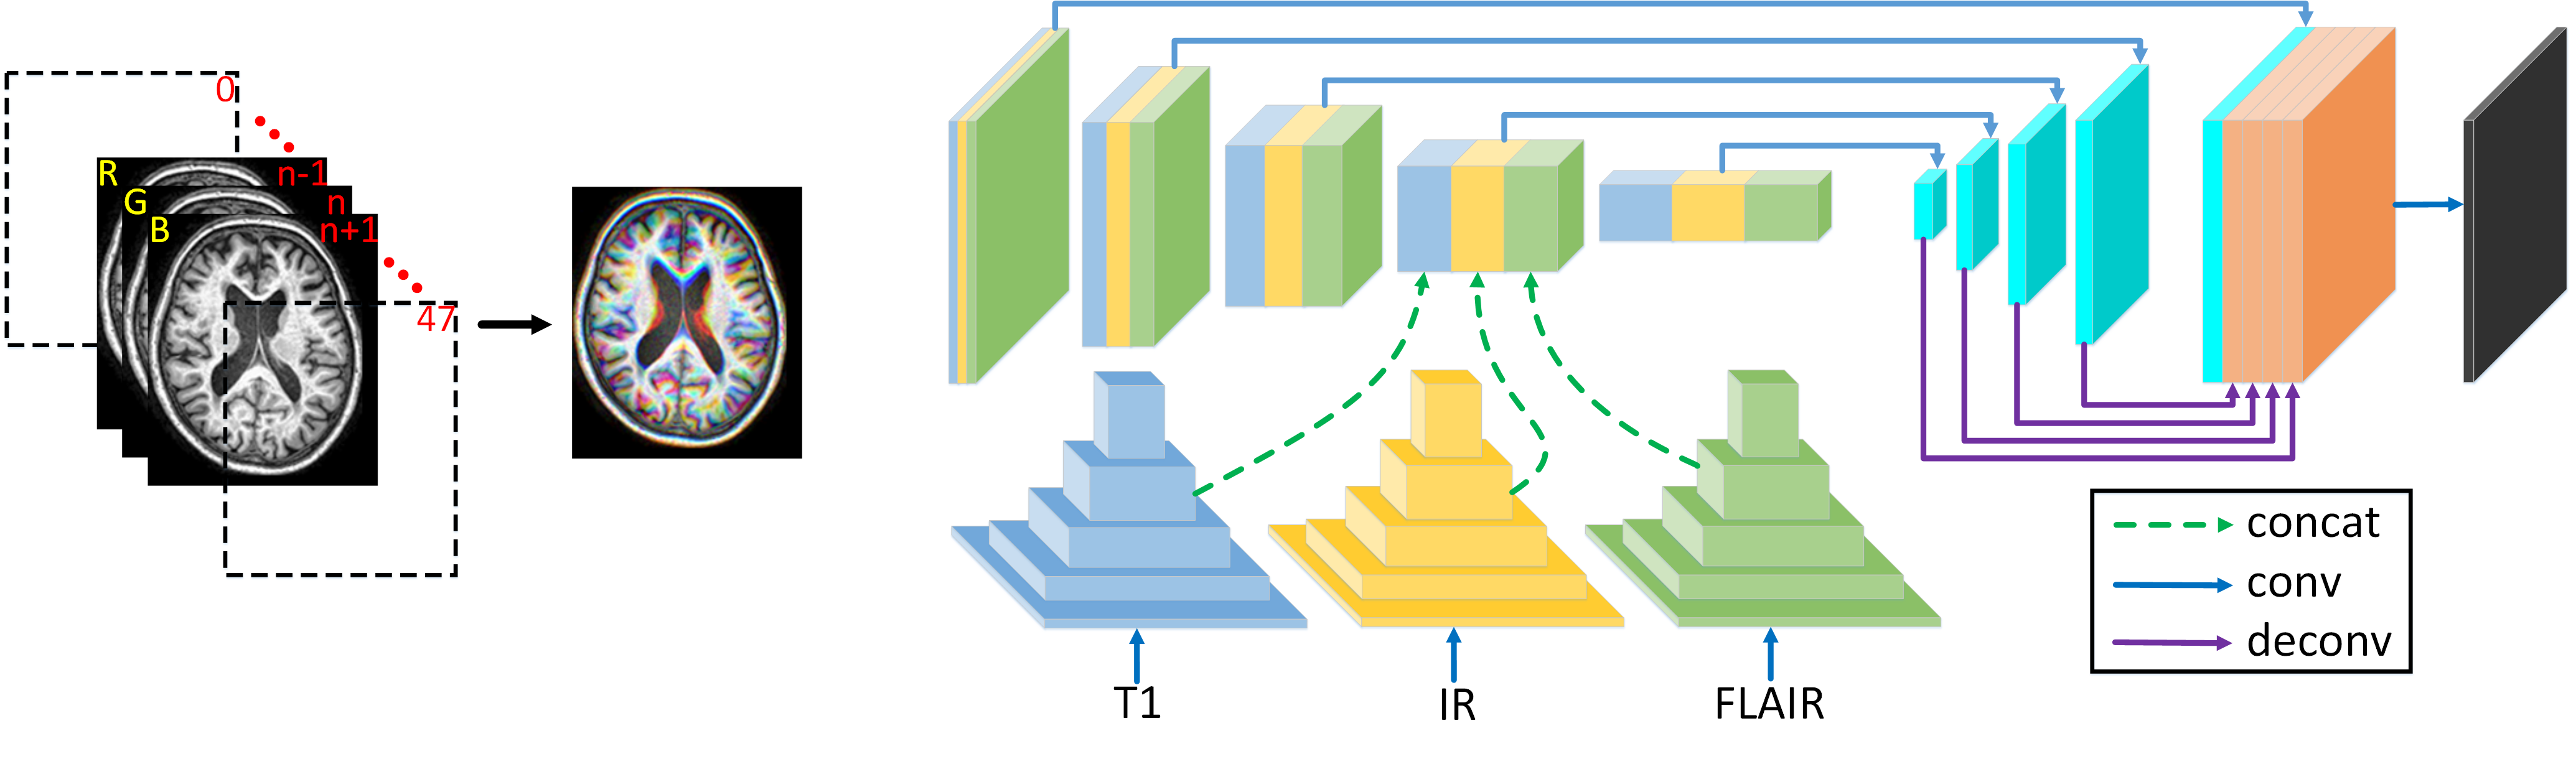
\includegraphics[width=\textwidth]{./imgs/pipeline.png}
    \caption{pipeline}
    \label{fig:pipeline}
\end{figure}

We use a HED-like\cite{Xie2016Holistically} FCN structure with 3$\times$ VGG16 as backbone, with carefully preprocessing. 
We use preprocessed T1,IR,FLAIR volumes. 

\textbf{Problems}:
\begin{itemize}
    \item ~The edge at the tissue boundary is not clear. 
    \item ~Some small organizations are difficult to segment.
    \item ~There are many neighbors between different organizations.
\end{itemize}

\textbf{Conclusions}:
\begin{itemize}
    \item ~Shallow network works much better than deep network. 
    \item ~Transfer learning plays a big role. 
    \item ~Multimodal image have great benefits for segmenting CSF and GM.
\end{itemize}

\textbf{Preprocessing}(shown in \ref{fig:preprocess}):
\begin{itemize}
    \item ~histogram equalization(only for T1);
    \item ~stack 3 continue slices as a RGB image;
    \item ~rotate for [$0,\pm 5,\pm 10,\pm 15$] for data augmentation;
    \item ~crop to reduce background in image and ensure width and height can be devided by 16;
\end{itemize}


\textbf{Pipeline}:
Following \cite{xu2017neonatal}, which is a HED-like\cite{Xie2016Holistically} structure. 
It is an simple and efficient decoder, which can handle little object better. 
Simply pass image in 3 modalities through 3 streams of VGG, and concat them in every stage, shown in \ref{fig:pipeline}. 

\begin{figure}[H]
    \centering
    \subfigure[source]{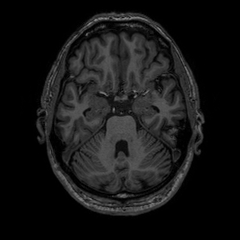
\includegraphics[scale=0.35]{./imgs/pre-src.png}}
    \subfigure[hist equalized]{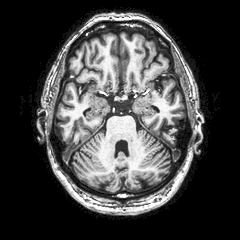
\includegraphics[scale=0.35]{./imgs/pre-eq.png}}
    \subfigure[stack 3 imgs]{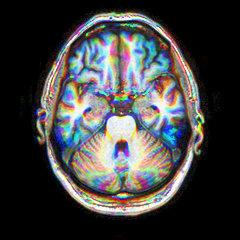
\includegraphics[scale=0.35]{./imgs/pre-rgb.png}}
    \subfigure[rotate]{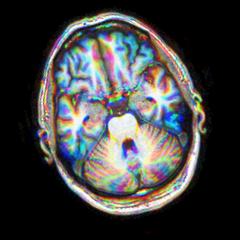
\includegraphics[scale=0.35]{./imgs/pre-rot.png}}
    \subfigure[crop]{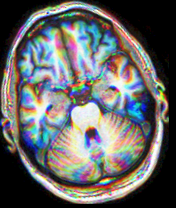
\includegraphics[scale=0.35]{./imgs/pre-crop.png}}
    \caption{preprocess}
    \label{fig:preprocess}
\end{figure}

\textbf{Parameters}:
\begin{itemize}
    \item ~Total number of iterations: 80k. 
    \item ~$\mathit{loss} : CrossEntropy$, $\mathit{optimizer} : SGD$.
    \item ~$\mathit{base\_lr} : 10^{-3}$, $\mathit{lr\_decay} : 0.1/4k$ iterations. 
    \item ~$\mathit{momentum} : 0.99$.
    \item ~$\mathit{weight\_decay} : 0.0005$. 
\end{itemize}

\textbf{LOSO Results}:

\begin{center}
\begin{tabular}{|c|c|c|c|}
    \hline
    {\bf Dice} & {\bf CSF} & {\bf GM} & {\bf WM}\\
    \hline
    {3*VGG16}          & \color{red}\bf{0.8247} & \color{red}\bf{0.8353} & \color{red}\bf{0.8663}\\
    {VGG16}            & \color{blue}{0.8053} & \color{blue}{0.8203} & \color{blue}{0.8628} \\
    {without transfer} & 0.7821 & 0.7995 & 0.8457 \\
    {Resnet50}         & 0.7808 & 0.7896 & 0.8179 \\
    \hline
\end{tabular}
\end{center}



\bibliography{cite}
\end{spacing}
\end{document}
